% \subsection{Pre-computation of mismatch values for hamming distance computation (IHD)}
\subsection{Improved Hamming distance computation by pre-computation of mismatch values (IHD)}
The EMS-GT2 uses the hamming distance computation heavily during the Test phase. As discussed earlier for the original EMS-GT, the hamming distnace of two binary represented $l$-mers, can be efficiently computed usign the boolean operator XOR. In EMS-GT2, instead of repeatedly counting this non-zero pairs of bits every time we compute the hamming distance, we use a pre-computed lookup table to help reduce computational time. Figure \ref{fig:pre-computed-hd} shows a snapshot of this table of pre-computed number of non-zero pairs of bits.

\begin{figure}[h]
	\centering
	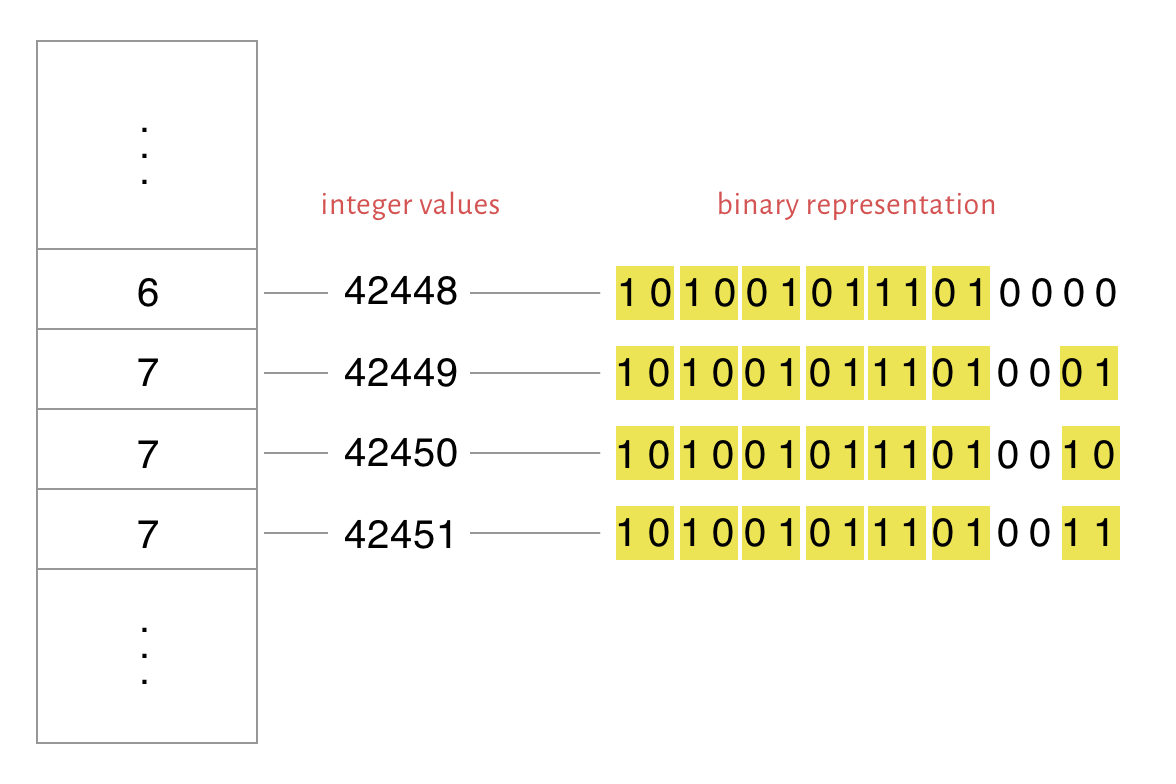
\includegraphics[width=4.0in]{contents/00_images/pre-computed-hd-values}\vspace*{5pt}
	
	\caption{An illustration of the pre-computed number non-zero pairs of bits up to a certain integer value for the hamming distance value computation.}
	\label{fig:pre-computed-hd}
\end{figure}

A naive pre-computation of these nonzero pair counts for all possible $l$-mers (each represented by 2$l$ bit values) will introduce an unacceptable overhead computation time when $l$ is sufficiently large, i.e., when $l \geq 10$ (based on actual runs on our current machine configurations). A more efficient approach is to pre-compute only up to $l$-mers of length $l' < l$, which required $b = 2l'$ number of bits. Then we determine the hamming distance by looking up to the nonzero counts in the XOR results, b number of bits at a time, as described in Algorithm 1. To illustrate the new process, Figure \ref{fig:usage-improved-hd} shows a demonstration of the improved hamming distance computation.

\begin{figure}[h]
	\noindent \hspace*{6pt}{\bf Algorithm 4} \textsc{Hamming Distance Computation using Pre-Computed Mismatch Values}
	\begin{algorithmic}[1]
		\label{alg:upd-hamming-distance-comp}
		\Require $l$-mer mappings $u$ and $v$ and\newline
			\hspace*{8pt} MC \Comment{array of pre-computed count of mismatch positions}
		\Ensure Hamming distance $d_H(u,v)$ \vspace*{6pt}
		\State $d_H(u, v) \leftarrow 0$
		\State $z \leftarrow u \oplus v$
		\While{$z > 0$}
			\State $l \leftarrow z \& ((1 << 18) - 1)$
			\State $d_H(u, v) \leftarrow d_H(u, v) + MC[l]$ 
			\State $z \leftarrow z >>> 18$ \Comment{shift 18 bits to the right}
		\EndWhile
		\State\Return $d_H(u, v)$
	\end{algorithmic}
\end{figure} 

\begin{figure}[h]
	\centering
	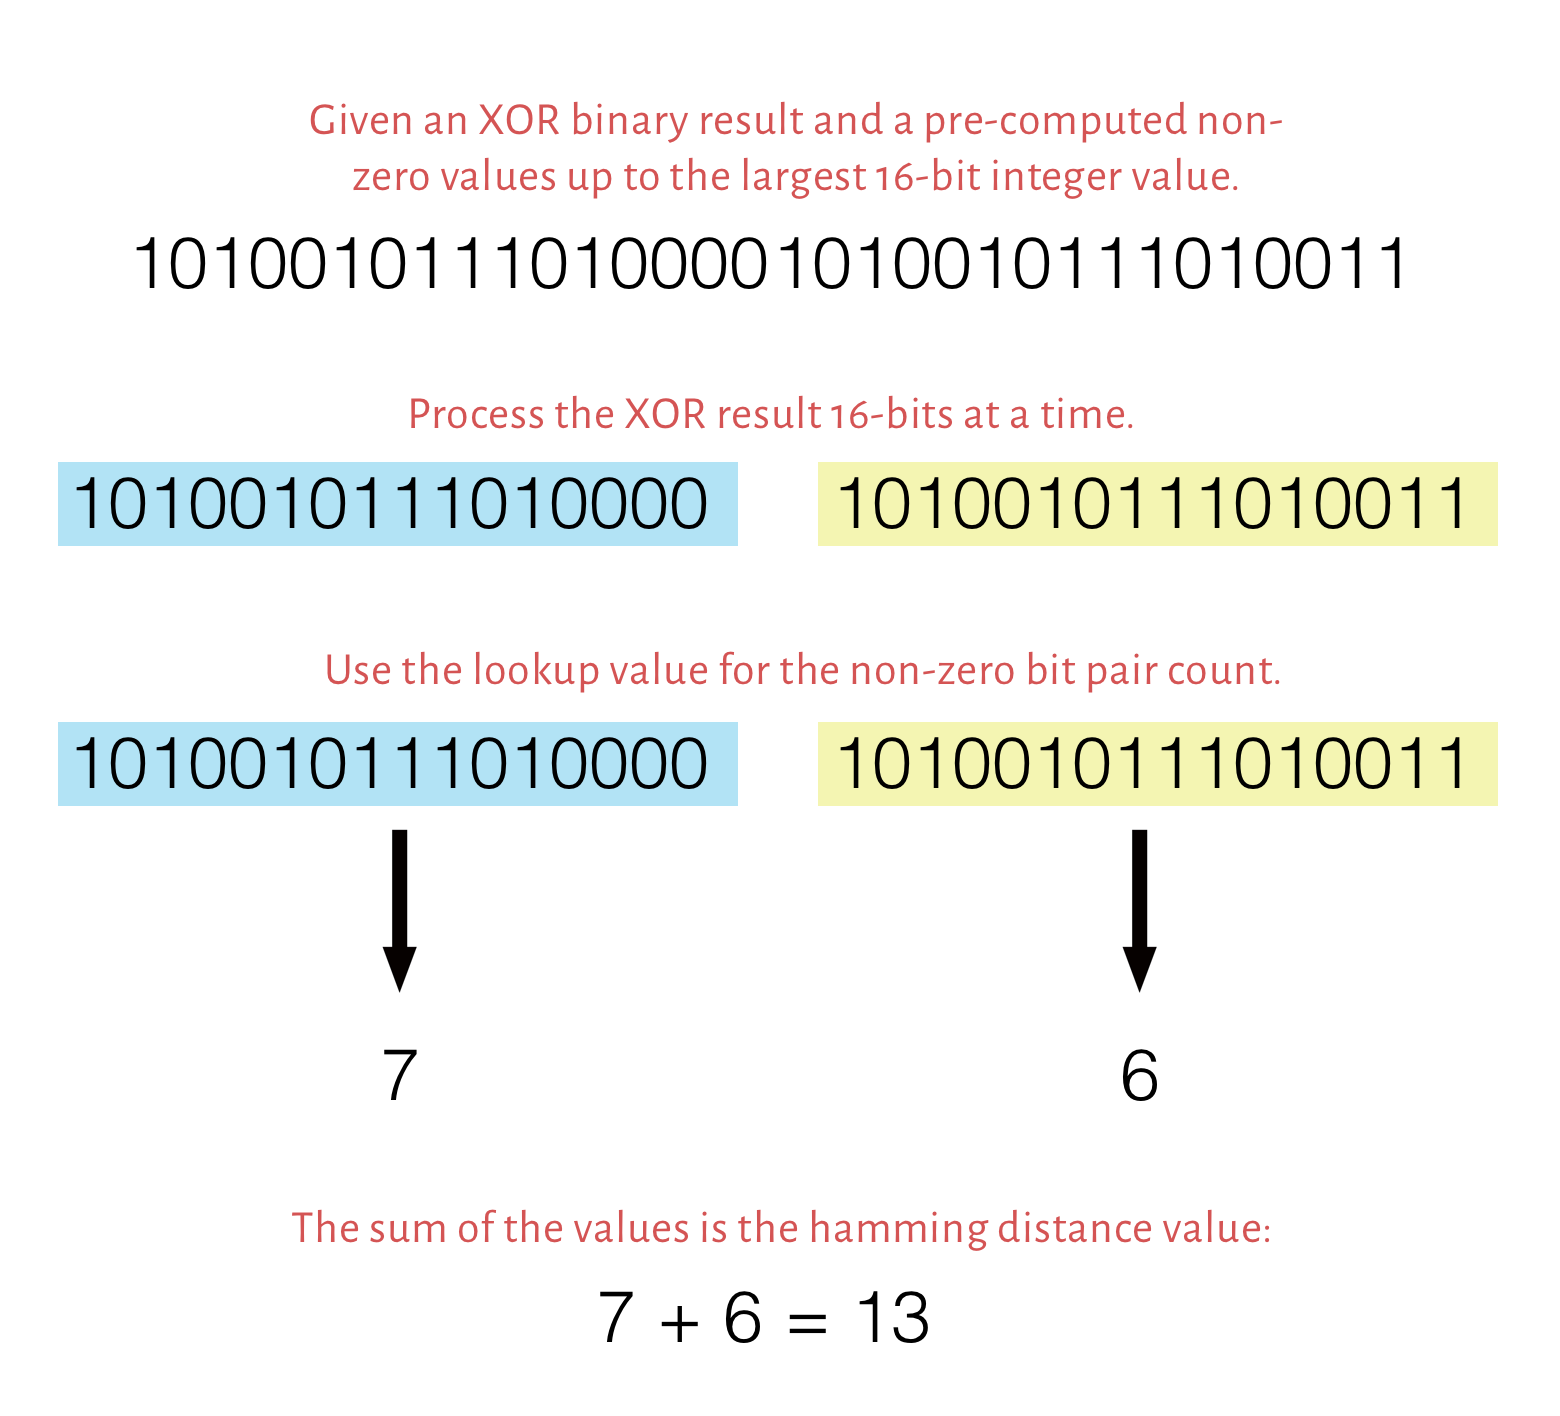
\includegraphics[width=4.0in]{contents/00_images/usage-improved-hd}\vspace*{5pt}
	
	\caption{A demonstration of the improved hamming distance value computation.}
	\label{fig:usage-improved-hd}
\end{figure}

In our experimentation the maximum required bits to represent $l$-mers is 34 bits (for (17, 6)-instance). Given this, we pre-compute up to 18 bits ($l' = 9$) values only and use the lookup table twice for the computation of the actual hammign distance between any given pair of $l$-mers.







